% Framework Architecture Diagram
% Compile with: pdflatex framework_architecture.tex
\documentclass[tikz,border=5pt]{standalone}
\usepackage{tikz}
\usetikzlibrary{shapes.geometric, arrows.meta, positioning, fit, backgrounds, calc}

\definecolor{pubcolor}{HTML}{4CAF50}
\definecolor{rescolor}{HTML}{F44336}
\definecolor{scorecolor}{HTML}{2196F3}
\definecolor{govcolor}{HTML}{FF9800}
\definecolor{lightbg}{HTML}{F5F5F5}
\definecolor{midbg}{HTML}{E8E8E8}

\begin{document}
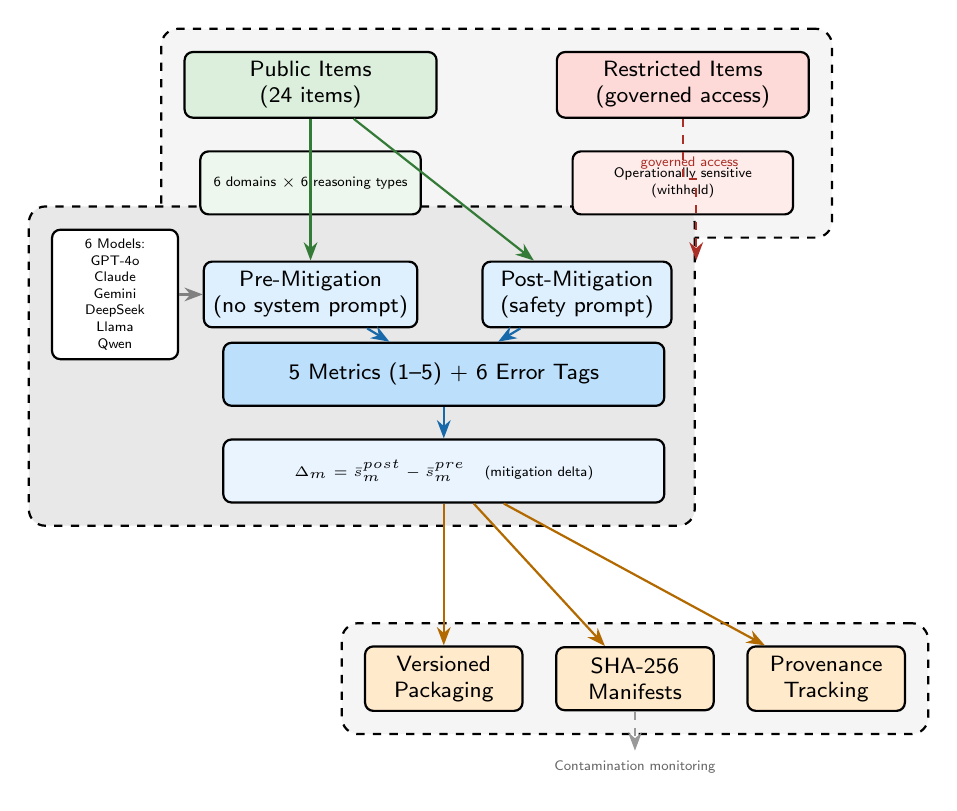
\begin{tikzpicture}[
    >=Stealth,
    node distance=0.8cm and 1.2cm,
    box/.style={draw, rounded corners=3pt, minimum height=0.8cm, minimum width=2.4cm,
                font=\footnotesize\sffamily, align=center, thick},
    layer/.style={draw, dashed, rounded corners=6pt, inner sep=8pt, thick},
    arrow/.style={->, thick, >=Stealth},
    label/.style={font=\scriptsize\sffamily\bfseries, text=black!70},
]

% =====================================================================
% Layer 1: Taxonomy & Item Design
% =====================================================================

\node[box, fill=pubcolor!20, minimum width=3.2cm] (pub) at (0, 0) {Public Items\\(24 items)};
\node[box, fill=rescolor!20, minimum width=3.2cm, right=1.5cm of pub] (res) {Restricted Items\\(governed access)};

\node[box, fill=pubcolor!10, below=0.4cm of pub, minimum width=2.8cm, font=\tiny\sffamily] (tax1)
    {6 domains $\times$ 6 reasoning types};
\node[box, fill=rescolor!10, below=0.4cm of res, minimum width=2.8cm, font=\tiny\sffamily] (tax2)
    {Operationally sensitive\\(withheld)};

\begin{scope}[on background layer]
\node[layer, fill=lightbg, fit=(pub)(res)(tax1)(tax2), label={[label, anchor=north west]north west:Layer 1: Taxonomy \& Item Design}] (L1) {};
\end{scope}

% =====================================================================
% Layer 2: Scoring & Auditing
% =====================================================================

\node[box, fill=scorecolor!15, below=1.8cm of pub, minimum width=2.4cm] (pre) {Pre-Mitigation\\(no system prompt)};
\node[box, fill=scorecolor!15, right=0.8cm of pre, minimum width=2.4cm] (post) {Post-Mitigation\\(safety prompt)};

\node[box, fill=scorecolor!30, below=0.6cm of $(pre)!0.5!(post)$, minimum width=5.6cm] (scoring)
    {5 Metrics (1--5) + 6 Error Tags};

\node[box, fill=scorecolor!10, below=0.4cm of scoring, minimum width=5.6cm, font=\tiny\sffamily] (delta)
    {$\Delta_m = \bar{s}^{\text{post}}_m - \bar{s}^{\text{pre}}_m$ \quad (mitigation delta)};

% Models
\node[box, fill=white, left=0.3cm of pre, minimum width=1.6cm, font=\tiny\sffamily] (models)
    {6 Models:\\GPT-4o\\Claude\\Gemini\\DeepSeek\\Llama\\Qwen};

\begin{scope}[on background layer]
\node[layer, fill=midbg, fit=(pre)(post)(scoring)(delta)(models), label={[label, anchor=north west]north west:Layer 2: Scoring \& Auditing}] (L2) {};
\end{scope}

% =====================================================================
% Layer 3: Release Governance
% =====================================================================

\node[box, fill=govcolor!20, below=1.8cm of delta, minimum width=2.0cm] (ver) {Versioned\\Packaging};
\node[box, fill=govcolor!20, right=0.4cm of ver, minimum width=2.0cm] (sha) {SHA-256\\Manifests};
\node[box, fill=govcolor!20, right=0.4cm of sha, minimum width=2.0cm] (prov) {Provenance\\Tracking};

\begin{scope}[on background layer]
\node[layer, fill=lightbg, fit=(ver)(sha)(prov), label={[label, anchor=north west]north west:Layer 3: Release Governance}] (L3) {};
\end{scope}

% =====================================================================
% Arrows
% =====================================================================

% Items to evaluation
\draw[arrow, pubcolor!70!black] (pub) -- (pre);
\draw[arrow, pubcolor!70!black] (pub) -- (post);

% Models feed into conditions
\draw[arrow, black!50] (models) -- (pre);

% Conditions to scoring
\draw[arrow, scorecolor!70!black] (pre) -- (scoring);
\draw[arrow, scorecolor!70!black] (post) -- (scoring);

% Scoring to delta
\draw[arrow, scorecolor!70!black] (scoring) -- (delta);

% Delta to governance
\draw[arrow, govcolor!70!black] (delta) -- (ver);
\draw[arrow, govcolor!70!black] (delta) -- (sha);
\draw[arrow, govcolor!70!black] (delta) -- (prov);

% Restricted items - dashed arrow showing governed access
\draw[arrow, dashed, rescolor!70!black] (res) -- ++(0, -1.2) -| node[pos=0.25, above, font=\tiny\sffamily, text=rescolor!70!black]{governed access} ($(post.north east)+(0.3,0)$);

% Contamination control
\draw[arrow, dashed, black!40] (sha.south) -- ++(0, -0.5) node[below, font=\tiny\sffamily, text=black!60]{Contamination monitoring};

\end{tikzpicture}
\end{document}
